\documentclass[12pt]{article}

\usepackage{polski}
\usepackage[utf8]{inputenc}
\usepackage{amsmath}
\usepackage{graphicx}
\usepackage[unicode]{hyperref}
\usepackage[utf8]{inputenc}
\usepackage{amsfonts}
\usepackage{physics}
\usepackage{graphicx}
\graphicspath{ {./images/} }

\title{4.1 Równanie transportu ciepła}
\author{Jakub Kędra}
\date{2023-01-23}

\begin{document}

\maketitle

% Wstęp

\section{Problem}

Celem projektu jest rozwiązanie metodą elementów skończonych poniższego równania różniczkowego

\begin{equation} \label{eq:main}
    -k(x) u''(x) = 100x
\end{equation}
% 
\text{dla warunków brzegowych:}
\begin{equation} \label{eq:statements}
    \begin{cases}
        u(2) = 0 \\
        u'(0) + u(0) = 20
    \end{cases}
\end{equation}
% 
\text{gdzie:} 
\begin{equation}
    k(x) = 
    \begin{cases}
        x + 1 & \text{dla } x \in [0,1]\\
        2x & \text{dla } x \in (1,2]
    \end{cases}
\end{equation}
% 
\text{oraz dla poszukiwanej funkcji $u$ takiej, że:}
\begin{equation}
    [0,2] \ni x \mapsto  u(x) \in \mathbb{R}   
\end{equation}


\section{Sformułowanie wariacyjne}

Zacznijmy od sformułowania wariacyjnego. Najpierw przekształćmy warunki brzegowe (\ref{eq:statements}) do wygodnej postaci:

\begin{equation} 
    \begin{cases}
        u(2) = 0 \\
        u'(0) = 20 - u(0) 
    \end{cases}
\end{equation}
% 
Ponieważ 
\begin{equation}
    \forall_{x\ \in\ \Omega}\ k(x) > 0  
\end{equation}
obie strony równania (\ref{eq:main}) możemy podzielić przez $k(x)$ 

\begin{equation}
    -u''(x) = \frac{100x}{k(x)}
\end{equation}
% 
Następnie równanie to musimy przemnożyć przez funkcję sprawdzającą $v(x)$, taką że:

\begin{equation}
    v \in V = \left\{f \in H^1(\Omega) : f(2) = 0 \right\}
\end{equation}
% 
\text{oraz zcałkować po obszarze $\Omega = (0,2)$:}

\begin{equation}
    \int_{0}^{2} -u''(x) v(x) dx = \int_{0}^{2} \frac{100x}{k(x)} v(x) dx
\end{equation}
% 
\text{Kolejnym krokiem jest rozpisanie funkcji $k(x)$:}

\begin{equation}
    \int_{0}^{2} -u''(x) v(x) dx 
    = \int_{0}^{1} \frac{100x}{x+1} v(x) dx
    + \int_{1}^{2} \frac{100x}{2x} v(x) dx
\end{equation}
% 
Po uproszeczeniu:
\begin{equation}
    \int_{0}^{2} -u''(x) v(x) dx 
    = \int_{0}^{1} \frac{100x}{x+1} v(x) dx
    + 50\int_{1}^{2} v(x) dx
\end{equation}
% 
Następnie obliczamy całkę pomocniczą:
\begin{equation}
    \begin{split}
        \int -u''(x) v(x) dx 
        & = \begin{vmatrix}
            t = v(x) & t' = v'(x) \\
            l' = -u''(x) & l = -u'(x)
        \end{vmatrix} = \\
        & = -v(x)u'(x) + \int v'(x) u'(x) \\
    \end{split}
\end{equation}
% 
I podstawiamy ją do równania:

\begin{equation}
    \eval{-v(x)u'(x)}_0^2 
    % 20v(0) - v(0)
    + \int_0^2 v'(x) u'(x) dx
    = \int_{0}^{1} \frac{100x}{x+1} v(x) dx
    + 50\int_{1}^{2} v(x) dx
\end{equation}

\begin{equation}
    - \underbrace{v(2)u'(2)}_0
    + v(0)\underbrace{u'(0)}_{20 - u(0)}
    + \int_0^2 v'(x) u'(x) dx
    = \int_{0}^{1} \frac{100x}{x+1} v(x) dx
    + 50\int_{1}^{2} v(x) dx
\end{equation}
% 
Po uwzględnieniu warunków brzegowych otrzymujemy równanie:
\begin{equation} \label{eq:finish}
    20v(0)
    - v(0)u(0)    
    + \int_0^2 v'(x) u'(x) dx
    = 
    \int_{0}^{1} \frac{100x}{x+1} v(x) dx
    + 50\int_{1}^{2} v(x) dx
\end{equation}
% 
Po pogrupowaniu elementów, otrzymujemy ostateczne równanie:
\begin{equation} \label{eq:finish}
    \underbrace{
        - v(0)u(0)    
        + \int_0^2 v'(x) u'(x) dx
    }_{B(u,v)}
    = 
    \underbrace{
        \int_{0}^{1} \frac{100x}{x+1} v(x) dx
        + 50\int_{1}^{2} v(x) dx
        - 20v(0)
    }_{L(v)}
\end{equation}
Na bazie którego konstruujemy funkcje $B(u,v)$ oraz $L(v)$
\section{Konstruowanie podprzestrzeni elementów skończonych $V_h \subset V$}
\subsection{Podprzestrzeń $V_h$}
Skoro po prawej stronie mamy warunek Dirichleta, a po lewej nie, za przestrzeń w której będziemy rozwiązywac ten problem przyjmujemy
\begin{equation}
    V_h = \langle e_0, e_1, e_2, ..., e_{n-1}\rangle
\end{equation}
% 
\subsection{Konstruowanie macierzy}
Równanie liniowe w postaci macierzowej do którego sprowadza się odnalezienie
\begin{equation}
    u = u_0e_0 + u_1e_1 + u_2e_2 + ... + u_{n-1}e_{n-1} \in V_h
\end{equation}
% 
spełniającego równanie (\ref{eq:finish}) dla każdego $v \in V_h$ ma zatem postać

\begin{equation}
    \begin{bmatrix}
        B(e_0,e_0) & B(e_0,e_1) & B(e_0,e_2) & \cdots & B(e_0,e_{n-1}) \\
        B(e_1,e_0) & B(e_1,e_1) & B(e_1,e_2) & \cdots & B(e_1,e_{n-1}) \\
        B(e_2,e_0) & B(e_2,e_1) & B(e_2,e_2) & \cdots & B(e_2,e_{n-1}) \\
        \vdots & \vdots & \vdots & \ddots & \vdots \\
        B(e_{n-1},e_0) & B(e_{n-1},e_1) & B(e_{n-1},e_2) & \cdots & B(e_{n-1},e_{n-1}) 
    \end{bmatrix}  
    \begin{bmatrix}
        u_0 \\
        u_1 \\
        u_2 \\
        \vdots \\
        u_{n-1}
    \end{bmatrix} 
    =
    \begin{bmatrix}
        L(e_0) \\
        L(e_1) \\
        L(e_2) \\
        \vdots \\
        L(e_{n-1})
    \end{bmatrix}
\end{equation}

\subsection{Funkcje bazowe}
W celu rozwiązania problemu wykorzystamy funkcje bazowe, zadane wzorem:
\begin{equation} \label{eq:defaultBasis}
    e_i = \begin{cases}
        \frac{x - x_{i-1}}{x_i - x_{i-1}} & \text{dla } x \in [x_{i-1}, x_i] \\
        \frac{x_{i+1} - x}{x_{i+1} - x_i} & \text{dla } x \in [x_i, x_{i+1}] \\
        0 & \text{wpp.}
    \end{cases}
\end{equation}
% 
Wzór ten możemy uprościć. Obliczmy różnicę pomiędzy poszczególnymi $x_i$:
\begin{equation}
    \Delta x = x_i - x_{i-1} = x_{i+1} - x_i
\end{equation}
% 
Niech
\begin{equation}
    \Delta x = h = \frac{b - a}{n}
\end{equation}
Gdzie:
\begin{itemize}
    \item $a,b$ oznacza początek i koniec obszaru $\Omega$ ($\Omega = (0,2) = (a,b)$)
    \item $n$ - liczbę elementów skończonych
\end{itemize}
% 
Z powyższych równań wynika, że: 
\begin{gather}
    x_{i-1} = x_i - h \\
    x_{i+1} = x_i + h
\end{gather}
% 
Po podstawieniu do wzoru (\ref{eq:defaultBasis}), otrzymujemy finalny wzór na $i$-tą funkcję bazową:
\begin{equation}
    e_i = \begin{cases}
        \frac{x}{h} - \frac{x_i}{h} + 1 & \text{dla } x \in (x_i - h, x_i] \\
        \frac{-x}{h} + \frac{x_i}{h} + 1 & \text{dla } x \in (x_i, x_i+h) \\
        0 & \text{wpp.}
    \end{cases}
\end{equation}
% 
A także jej różniczkę:
\begin{equation}
    e_i = \begin{cases}
        \frac{1}{h} & \text{dla } x \in (x_i - h, x_i] \\
        -\frac{1}{h} & \text{dla } x \in (x_i, x_i+h) \\
        0 & \text{wpp.}
    \end{cases}
\end{equation}

\section{Program}
\subsection{Wykres (dla n = 1000)}
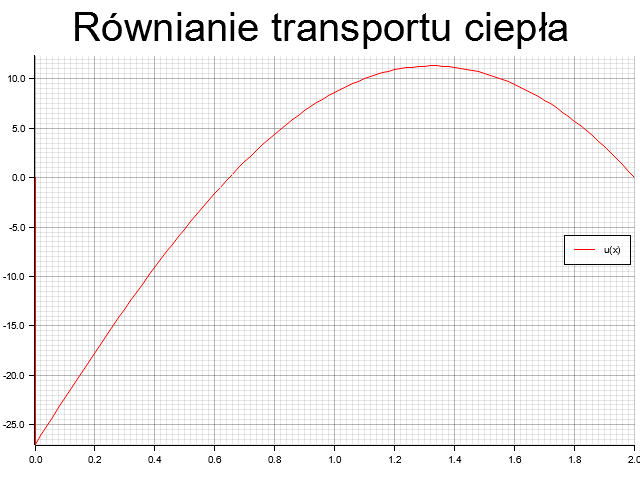
\includegraphics[width=\textwidth,height=\textheight,keepaspectratio]{plot.png}


\subsection{Kompilacja}
Program został napisany w języku Rust. Aby go skompilować, w katalogu głównym aplikacji należy uruchomić polecenie
\begin{verbatim}
cargo build --release
\end{verbatim}
Skompilowany program znajduje się wewnątrz katalogu target/release

\subsection{Uruchomienie}
Przygotowany, skomilowany program znajduje się wewnątrz katalogu build.
Aby uruchomić aplikację, należy z poziomu konsoli uruchomić polecenie:
\begin{verbatim}
.\fem.exe <n> <output>
\end{verbatim}
gdzie
\begin{itemize}
    \item n - wymagany parametr n
    \item output - opcjonalny parametr, ścieżka do pliku wynikowego z wykresem, domyślnie output.png
\end{itemize}

\end{document}